\documentclass[reprint, english,notitlepage]{revtex4-1}  % defines the basic parameters of the document
% if you want a single-column, remove reprint

% allows special characters (including æøå)
\usepackage[utf8]{inputenc}
\usepackage [norsk]{babel} %if you write norwegian
%\usepackage[english]{babel}  %if you write english


%% note that you may need to download some of these packages manually, it depends on your setup.
%% I recommend downloading TeXMaker, because it includes a large library of the most common packages.

\usepackage{physics,amssymb}  % mathematical symbols (physics imports amsmath)
\usepackage{graphicx}         % include graphics such as plots
\usepackage{xcolor}           % set colors
\usepackage{hyperref}         % automagic cross-referencing (this is GODLIKE)
\usepackage{tikz}             % draw figures manually
\usepackage{listings}         % display code
\usepackage{subfigure}        % imports a lot of cool and useful figure commands
\usepackage{verbatim}
\usepackage{adjustbox}

% defines the color of hyperref objects
% Blending two colors:  blue!80!black  =  80% blue and 20% black
\hypersetup{ % this is just my personal choice, feel free to change things
    colorlinks,
    linkcolor={red!50!black},
    citecolor={blue!50!black},
    urlcolor={blue!80!black}}

%% Defines the style of the programming listing
%% This is actually my personal template, go ahead and change stuff if you want
\lstset{ %
	inputpath=,
	backgroundcolor=\color{white!88!black},
	basicstyle={\ttfamily\scriptsize},
	commentstyle=\color{magenta},
	language=Python,
	morekeywords={True,False},
	tabsize=4,
	stringstyle=\color{green!55!black},
	frame=single,
	keywordstyle=\color{blue},
	showstringspaces=false,
	columns=fullflexible,
	keepspaces=true}

\begin{document}



\title{Lab 2 - Strøm og spenning}
\date{\today}
\author{Candidate 073402}
\affiliation{FYS2150, University of Oslo}
\email{textme@lab.uio.no}


\newpage

\begin{abstract}
Jeg har studert lys som er observert fra en fjern stjerne på ti forskjellige dager over en toukers periode. Ved å se på Doppler-forskyvning av en spektrallinje har jeg klart å beregne stjernens hastighet i forhold til oss ved hver av de ti målingene. På bakgrunn av dette kunne jeg slå fast at stjernen beveger seg bort fra oss med en gjennomsnittshastighet på ca. 15km/s. Den beveger seg i tillegg i bane med svært kort omløpsperiode, bare rundt 10 dager, og høy banefart, ca. 1.5km/s. Dette indikerer tilstedeværelsen av et annet massivt legeme like i nærheten.

For å finne eksakte verdier for bølgelengden til absorpsjonslinjen i det Doppler-forskjøvede spekteret brukte jeg minste kvadraters metode. Termiske bevegelser i gassene på stjernens overflate, og annen støy, gjør at dette kan være vanskelig å gjøre med øyemål. Jeg har anvendt modeller for fluks og støy som bygger på normalfordelingen, noe som har vist seg å være fornuftige antakelser.
\end{abstract}
\maketitle                                % creates the title, author, date & abstract



\section{Introduksjon}

Måling av støm, spenning og motstand er svært sentralt i eksperimentell fysikk, ikke bare fordi kunnskap om disse størrelsene og måling av dem er viktige i seg selv, men også fordi instrumenter vi bruker til å måle mange andre størrelser ofte gir elektriske signaler som vi må tolke. Dette gjelder både i vitenskapelige eksperimenter og i industrielle og praktiske anvendelser, eksempelvis temperatur og trykk.

Vi har i dette eksperimentet sett på egenskapene til multimetre som kan brukes til å måle både spenning, strøm og motstand. Vi har sett på forskjellen mellom å bruke multimetrene til å måle motstand direkte og i stedet måle strøm og spenning for siden å bruke Ohms lov til å beregne motstanden i kretsen. Til sist har vi brukt både multimetre og et oscilloskop til å studere elektrisk signal som er laget av en signalgenerator og brukt de samme redskapene til å se på forskjellige egenskaper ved en RC-krets.


\section{Teori}

Ved å observere lyset som når oss fra fjerne stjerner kan vi finne ut hvilken fart stjernen har i
 forhold til oss her på jorda. På grunn av Doppler-Effekten vil lys sendt ut fra en kilde som
 beveger seg bort fra oss bli rødforskjøvet og lys fra en kilde som beveger seg mot oss vil bli
 bl



\section{Eksperimentelt}

Vi har brukt to multimetre, Fluke 45 og Fluke 75, og brukt hver av dem til å måle på det andre. På den måten har vi målt motstand til et voltmeter og et amperemeter, strømmen og spenningen over et ohmmeter


\subsection{Vekselspenninger med frekvensgenerator, oscilloskop og multimeter}
De to signalene vi brukte i analysen var et sinus- og et firkantsignal. Bilder av signalene med innstillingene som ble brukt finnes i figur REF.

\begin{figure}
  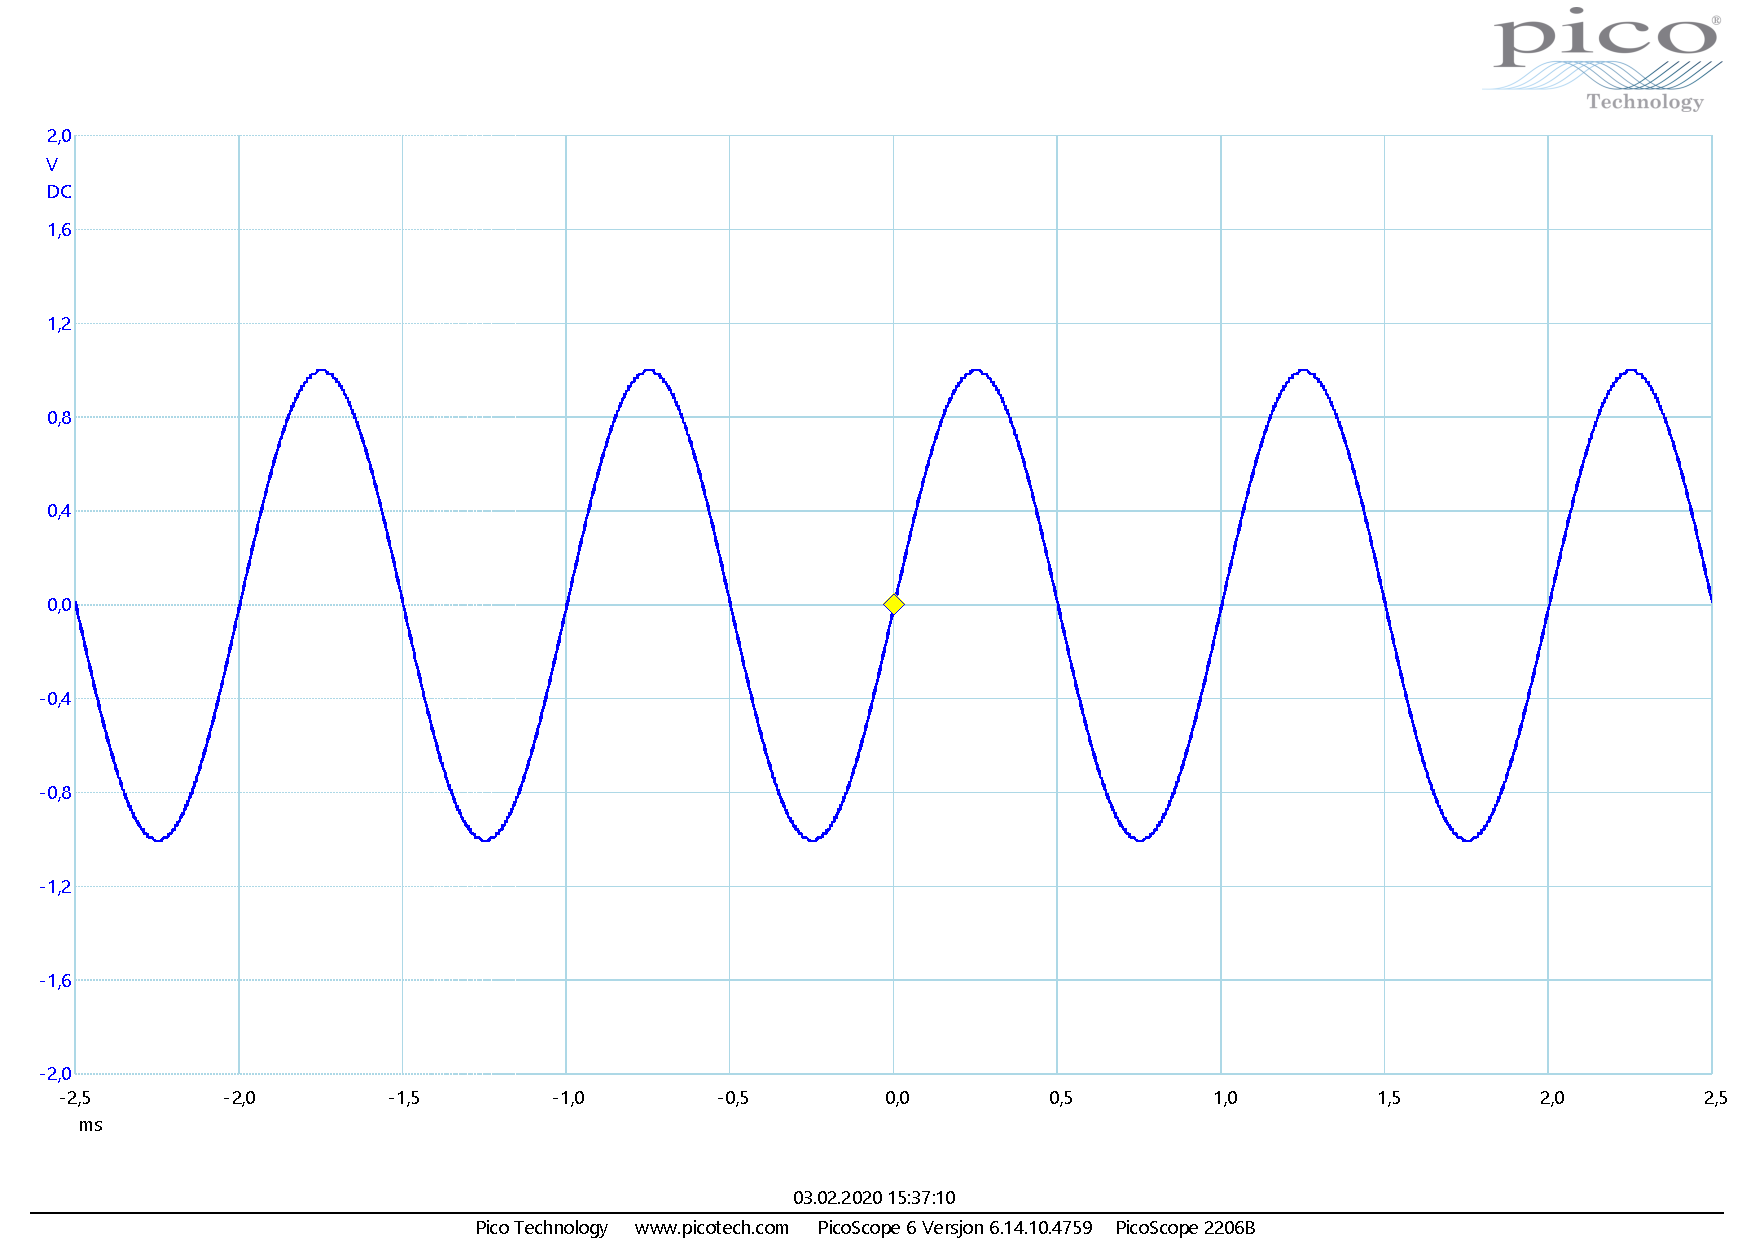
\includegraphics[width=\linewidth]{../sinus.pdf}
  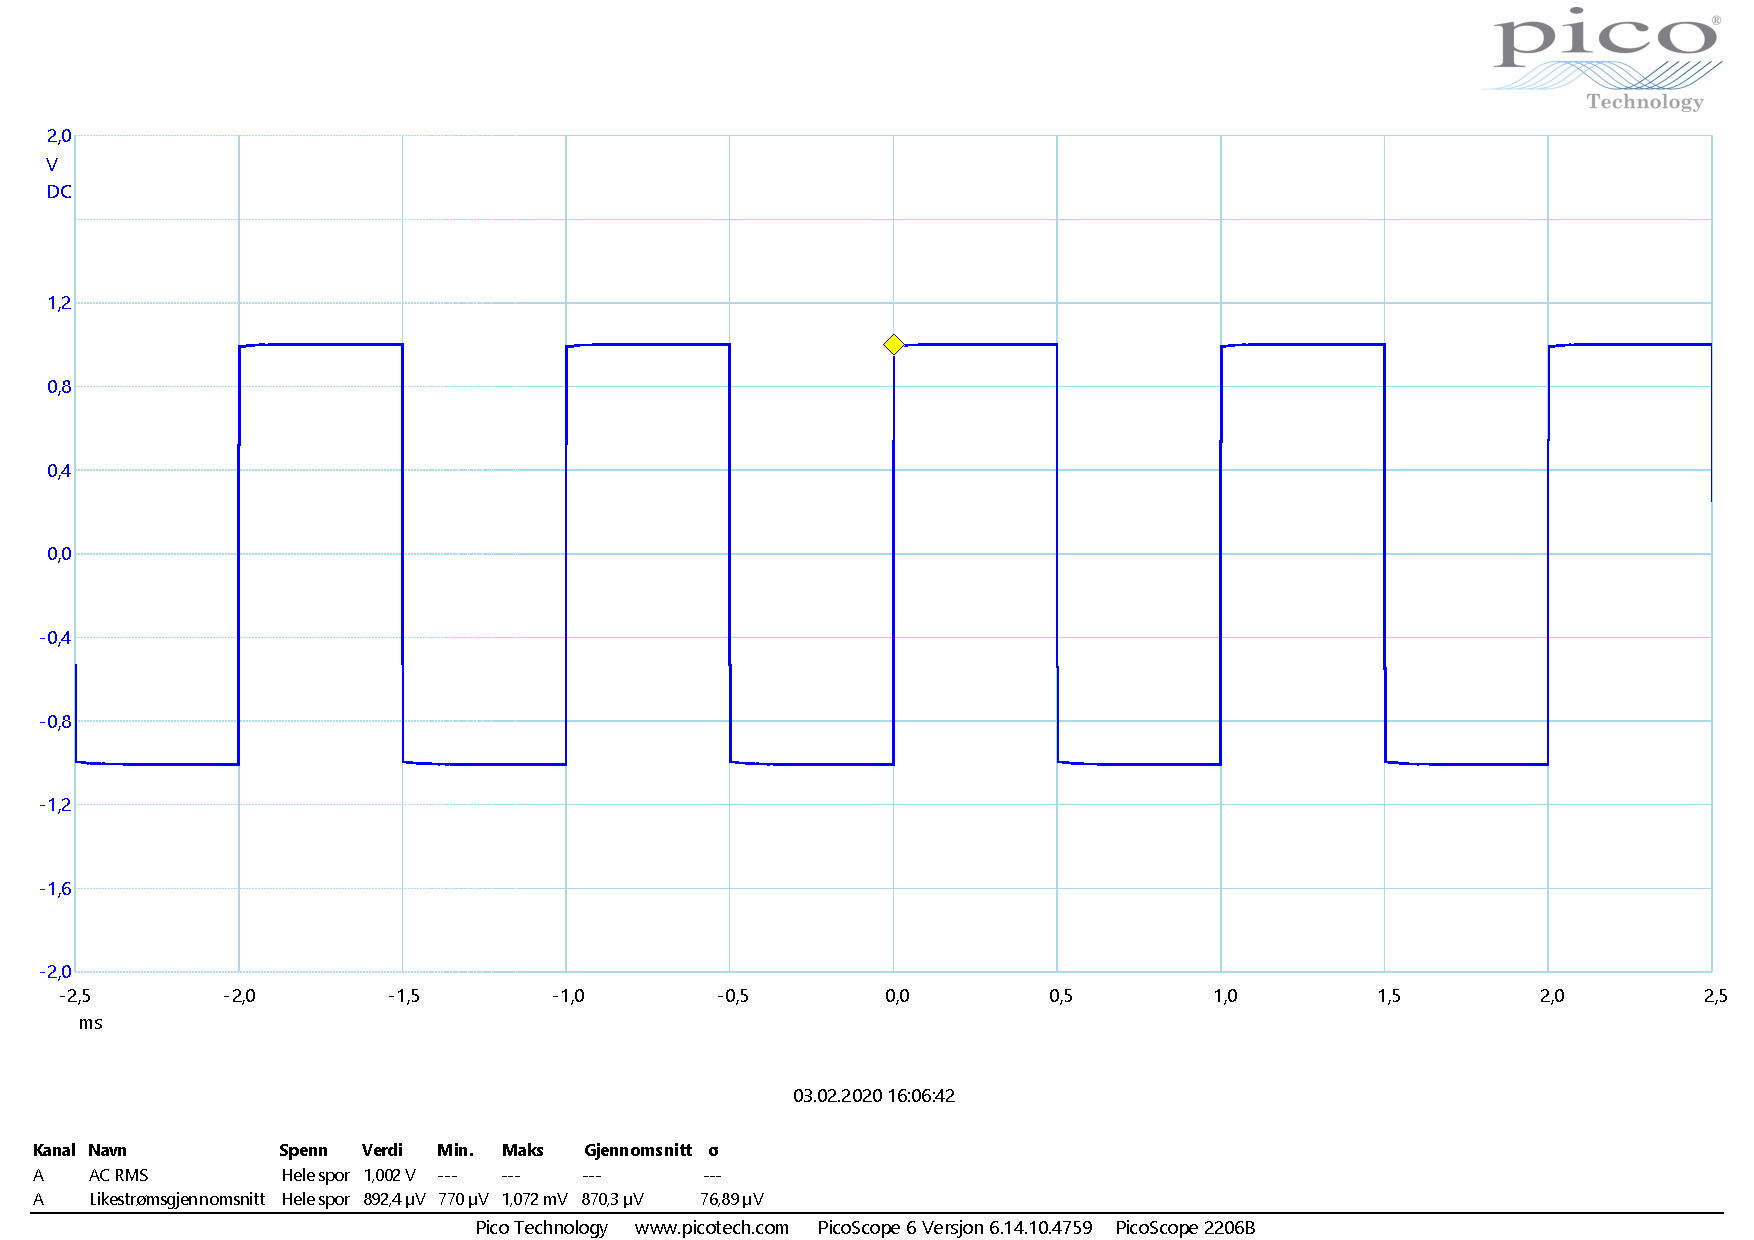
\includegraphics[width=\linewidth]{../firkant.pdf}
  \caption{Sinus- og firkantsignalet brukt til å måle vekselspenning med oscilloskop. Begge siganelene hadde en frekvens på 1 kHz og amplitude 1 V. Resten av innstillingene 500 $\mu$s/div, 1 MS, $\pm$ 2 V, AC, 12 bit.}
  \label{fig:sinussignal}
\end{figure}


\section{Resultater}

\subsection{Multimeter måler multimeter}
Den første delen av eksperimentet, å bruke hvert av multimetrene til å måle på det andre, ga resultatene presentert i tabell \ref{fig:tabell_multimetre}.

\begin{table}[p]
\label{fig:tabell_multimetre}
\caption{Tabell som viser resultatene av å bruke de to multimeterne til å måle på hverandre. Målingene merket med * var oppgitt med én desimal mer på måleinstrumentet enn det som er oppgitt her, men det siste sifferet er sløyfet fori det var umulig å avlese da verdien svingte hele tiden.}

\begin{adjustbox}{width=\linewidth}
\begin{tabular}{||c | c | c | c||}
\hline
Forsøk \# & Spenning, [mV] & Strøm, [mA] & Motstand  \\ \hline\hline
1 &            & F45: 0.501 & F75: 10.9 $\Omega$    \\ \hline
2 &            & F75: 0.81  & F45: 5.94             \\ \hline
3 & F45: 0.01  & F75: 0.00  &                       \\ \hline
4 & F75: 0.0   & F45: 0.000 &                       \\ \hline
5 & F45: 722.4 &            & F75: 10.03 M$\Omega$  \\ \hline
  &     1982.2 &            &        OL. $\Omega$   \\ \hline
  &     1979.3 &            &        OL $\Omega$    \\ \hline
  &     1426.4 &            &        O.L k$\Omega$  \\ \hline
  &     1310.0 &            &        OL. k$\Omega$  \\ \hline
  &      722.3 &            &        .OL  M$\Omega$ \\ \hline
6 & F75:  1552 &            & F45: 11.10 M$\Omega$*  \\ \hline
  &       1552 &            & 11.1 M$\Omega$*        \\ \hline
  &       1552 &            & 11.1 M$\Omega$         \\ \hline
\end{tabular}
\end{adjustbox}
\end{table}

Den første kretsen i figur REF svarer til Voltmeter-funksjonen. Den andre svarer til et Amperemeter, og den tredje er et Ohmmeter.


\subsection{Motstand, likestrøm og likespenningsmålinger med multimeter}
Ved å måle motstandene R1 og R2 direkte fikk vi disse verdiene:
\begin{itemize}
  \item R1 = 10.10 $\pm$ 0.01 $\Omega$
  \item R2 = 0.99 $\pm$ 0.02 M$\Omega$
\end{itemize}

Ved indirekte måling av motstanden ved Ohms lov fikk vi først verdiene for strøm og spenning som er vist i tabell REF. Ved likning REF fikk vi da disse verdiene for størrelsene på motstandene:
\begin{itemize}
  \item R1 = 10.37 $\pm 0.06 \Omega$
  \item R2 = 0.90 $\pm$ 0.07 M$\Omega$
\end{itemize}

\begin{table}[p]
\label{fig:tabell_motstander}
\caption{Tabell som viser resultatene av å bruke de to multimeterne til å måle strøm og spenning gjennom kretsene i figur REF. Målingen merket med * er avlest for tidlig i forhold til den tiden som multimeter bruker på å stabilisere seg når man måler strøm med største presisjon, og er ikke egnet til å brukes i videre beregninger.}

\begin{adjustbox}{width=\linewidth}
\begin{tabular}{||c | c | c | c||}
\hline
Komponent & Måling & Spenning, [V] & Strøm, [mA]   \\ \hline\hline
R1 & Spenning inn     & 1.474 $\pm$ 0.007 & 68.93 $\pm$ 0.04*   \\ \hline
   & Spenning over R1 & 0.716 $\pm$ 0.004 & 69.01 $\pm$ 0.04    \\ \hline
R2 & Spenning inn     & 17.78 $\pm$ 0.08  & 0.018 $\pm$ 0.002   \\ \hline
   & Spenning over R2 & 17.79 $\pm$ 0.08  & 0.020 $\pm$ 0.002   \\ \hline
\end{tabular}
\end{adjustbox}
\end{table}

\subsection{Vekselspenninger med frekvensgenerator, oscilloskop og multimeter}
Ting og tang, og blablabla


\section{Diskusjon}

Når jeg analyserte fluksdataen med minste kvadraters metode bruke jeg 30 testverdier for hver av
 de ukjente parametrene $F_{\text{min}}$, $\sigma$ og $\lambda_{\text{center}}$. Ved å øke til 40 testverdier
 innenfor det samme intervallet forventet jeg å få mer nøyaktige svar. Det viste seg imidlertid
 at dette bare førte til en endring på mellom 0.00003\% og 0.00013\% av $\lambda_{\text{center}}$ som er
 den parameteren vi bryr oss om. Jeg konkluderer derfor med at 30 testverdier gir så godt som så
 presise svar vi kan finne, og jeg er komfortabel med å bruke 30 testverdier videre. Som nevnt i
 metode-delen oppdaget jeg etter implementering av algoritmen at den øvre grensen for $\sigma$
 trygt kunne vært satt en del lavere enn den verdien jeg brukte. Dette ville antakeligvis gitt
 noe mer nøyaktige resultater.

Ved å se på  vi tydelige periodiske svingninger i hastigheten til
 stjernen. Det betyr at stjernen beveger seg i bane og har en komponent av banehastigheten som er
 parallell med vår siktlinje. For at stjernen skal gå i bane, må den påvirkes av en
 gravita


\section{Konklusjon}
blablabla



\onecolumngrid
\vspace{1cm} % some extra space


\begin{thebibliography}{}
\bibitem[Hansen (2017)]{part1A} Hansen, F. K.,  2017, Forelesningsnotat 1A i kurset AST2000
\bibitem[Hansen (2017)]{part1C} Hansen, F. K.,  2017, Forelesningsnotat 1C i kurset AST2000
\bibitem[Hansen (2017)]{part1D} Hansen, F. K.,  2017, Forelesningsnotat 1D i kurset AST2000
\bibitem[15889 (2019)]{paper1C} 15889,  2019, Ekstrasolare planeter
\bibitem[5]{wiki} Solen, https://no.wikipedia.org/wiki/Solen, Lest 17.10.19

\end{thebibliography}



\section{Appendix}


\begin{table}[p]
\begin{adjustbox}{width=1\textwidth}
\begin{tabular}{||c | c | c | c | c||}
\hline
Day & $F_{\text{min}}$ & $\sigma$ & $\lambda$, [nm] & $\Delta$ \\ \hline\hline
0 & 0.81742 & 0.00438 & 656.33020 & 3.73793    \\ \hline
2 & 0.81084 & 0.00438 & 656.33422 & 3.55735    \\ \hline
3 & 0.81249 & 0.00438 & 656.33580 & 3.75985    \\ \hline
5 & 0.81334 & 0.00438 & 656.33498 & 3.69936    \\ \hline
6 & 0.79401 & 0.00438 & 656.33100 & 4.00017    \\ \hline
8 & 0.80051 & 0.00438 & 656.32920 & 3.65960    \\ \hline
9 & 0.80140 & 0.00438 & 656.33002 & 3.83682    \\ \hline
11 & 0.80581 & 0.00438 & 656.33418 & 3.88872    \\ \hline
13 & 0.80998 & 0.00438 & 656.33618 & 3.65010    \\ \hline
14 & 0.81709 & 0.00438 & 656.33440 & 3.68551    \\ \hline
\end{tabular}
\end{adjustbox}
\caption{Tabell som viser resultatene av minste kvadraters metode anvendt på dataen registrert for hver av de 10 dagene. $F^{\text{model}}$ er testet med alle kombinasjoner av 30 forskjellige verdier for $F_{\text{min}}$, $\sigma$ og $\lambda_{\text{center}}$. Den beste kombinasjonen ga totalt avvik $\Delta$ mellom $F^{obs}$ og $F^{\text{model}}$.}
\label{fig:table}
\end{table}



\end{document}
